\chapter{Propuesta de solución}

La propuesta detallada a continuacion tiene como consideracion los siguientes objetivos referentes a este trabajo:

\begin{itemize}
\item Establecer un marco de trabajo para la recolección, entrenamiento y clasificación de algoritmos de machine learning utilizando Bluetooth Lo Energy

\item Comparación de diferentes clasificadores, para determinar sus ventajas y cuales se comportan de mejor forma en la fase de entrenamiento y test, para asi seleccionar los mejores.

\item Utilizar técnicas de reducción de dimensionalidad para reducir la complejidad del problema, y optimizar los recursos para así disminuir el procesamiento de los dispositivos móviles.

\item Determinar los mejores valores para el funcionamiento correcto de los dispositivos Bluetooth en el contexto del posicionamiento en interiores.

\item Utilizar modelos sin necesidad de conexión a internet, es decir, solo utilizar redes Bluetooth sin siquiera tener habilitado el WI-Fi en dispositivos móviles o las redes LTE. Todo el procesamiento se realiza en el cliente, por lo que es importante utilizar algoritmos de gran desempeño y bajo procesamiento.
\end{itemize}


\section{Consideraciones Previas}

Para resolver el problema de la localización abarcado en esta memoria, hay muchas posibilidades las cuales presentan sus ventajas e inconvenientes con respecto a consumo de recursos, precisión, exactitud, tiempo de procesamiento, entre otros. Por lo mismo, para generar el \textit{framework} de localización,se requiere determinar las opciones factibles que presenten un equilibrio entre todos los parámetros anteriormente nombrados.

Como el objetivo principal de esta memoria es determinar que tan bien se comporta la tecnología \textit{Bluetooth Low Energy} desempeñando la labor de localización, en primer lugar es necesario comparar las diferentes alternativas existentes en el mercado relativas a esta tecnología, que presenten facilidad de uso, un precio relativamente módico y acceso a plataformas de desarrollo o \textit{software development kit} (SDK). A continuacion se detallan las principales caracteristicas de los Beacons Bluetooth y posteriormente se realiza una comparativa entre los dos proveedores mas grandes.

\subsection{Definición de beacons bluetooth y sus protocolos}

La definición mas básica de Beacon Bluetooth hace referencia a un dispositivo transmisor de ondas de radio Bluetooth. Estos equipos continuamente emiten señales que otros dispositivos pueden recibir mediante sensores adecuados. Lo que envían corresponde a señales de letras y numeros en forma de paquetes que se transmiten en intervalos regulares de aproximadamente 100 mili segundos. Dentro de los beacons existen placas madres que contienen una CPU, transmisor de radio, y baterias. Ademas pueden presentar acelerometro, sensores de temperatura, entre otros.

La transmision corresponde a un ID unico que esta presente en cada Beacon y que no se repite, como una direccion MAC o un UUID pertinente, dependiendo de cada fabricante. Este ID por si solo carece de sentido, ya que solo es una direccion, la manera mas practica en que son utilizados estos dispositivos es generar una infraestructura completa y asociar estos ID a posiciones o maquinarias para ser localizadas. Todo esto depende del uso y contexto en que se despliega la aplicación que utiliza los Beacons. Por lo mismo, todo lo que el Beacon transmite es utilizado por los programadores para sus propias necesidades, como enviar un mensaje o anuncio a un smartphone especifico, o generar localización en tiempo real.

A pesar de que esta tecnologia existe hace muchos años, últimamente se ha vuelto sumamente relevante por el auge del \textit{internet of things}(IOT). Con receptores Bluetooth en 90\% de los equipos móviles, esta tecnología es perfecta para emitir mensajes en un rango corto-medio y generar una completa infraestructura o ecosistema de redes conectadas en cualquier lugar del planeta. Ademas desde el 2010, el estandar corresponde a BLE o Bluetooth Low Energy, el cual corresponde a una version mucho mas eficiente energeticamente y que ha hecho posible el auge de los Beacons, ya que gracias a este estandar, solo se requiere pequeñas baterias para que estos dispositivos puedan emitir señales por meses e incluso años, lo que convierte a BLE en el mayor avance en IOT por su simplicidad y eficiencia.

\subsubsection{¿Como se comunican los Beacons?}

Los Beacons envian sus ID unicos aproximadamente 10 veces por segundo dependiendo de la configuracion, y cualquier dispositivo que se encuentre en su rango de alcance es capaz de reconocer este ID, como por ejemplo un telefono celular o un computador portatil. Cuando una aplicacion dedicada reconoce este ID, puede emitir un evento en el sistema operativo, como por ejemplo mostrar un mensaje, descargar un archivo de la web, o realizar un algoritmo de localizacion.

\subsubsection{¿Donde comenzo la tecnologia Beacon?}

Los Beacons como se conocen hoy en dia comenzaron con la creación de los reconocidos IBeacons, implementados por la compañía Apple. IBeacon es un protocolo simple que permite transmitir muy pequeñas porciones de datos. Posteriormente Google lanza su propio protocolo en 2015, denominado EddyStone, como una alternativa a IBeacon. A raiz de esto se ha generado una competencia que ha ayudado a mejorar el hardware y software de los dispositivos Beacons. A continuación se muestra una tablas con los parámetros basicos de cualquier dispositivo Beacon, que ayudan a mejorar su eficiencia sin perdida de precisión.

\begin{table}[]
\centering
\caption{My caption}
\label{my-label}
\begin{tabular}{|c|c|c|c|}
\hline
Intervalo & Tx Power   & Rango esperado & Bateria esperada \\ \hline
100ms     & 3(-12 dBm) & 35m            & Hasta 7 meses    \\ \hline
300ms     & 3(-12 dBm) & 35m            & Hasta 2 años     \\ \hline
1000ms    & 3(-12 dBm) & 35m            & Hasta 4 años     \\ \hline
\end{tabular}
\end{table}

Los parámetros de la tabla anterior se definen a continuacion:

\begin{itemize}
\item \textbf{Bateria esperada: } La mayoría de los Beacons tienen una duración esperada en su batería de 18 a 24 meses, sin embargo dependiendo de las configuraciones y usos su batería puede caer de 6 a 8 meses. Los Beacons con ahorro de energía pueden incluso llegar a 5 años de duración. La explicación en como pueden durar tanto, se basa en el protocolo Bluetooth Low Energy el cual es realmente eficiente.

\item \textbf{Formato soportado: } Habitualmente los Beacons soportan ambos protocolos, es decir IBeacon y Eddystone.

\item \textbf{Intervalo: } Representa que tan seguido los Beacons transmiten el mensaje. A pesar de que este numero puede ser sumamente bajo, la mayor parte de los sistemas operativos no permiten leer tan rapidamente con lo cual un valor menor a 100ms es innecesario en la mayoria de los casos.

\item \textbf{TX Power: } Este valor describe que tan lejos puede llegar la señal emitida por la radio del Beacon. Puede ser tan pequeña como 4 metros, pero habitualmente pueden llegar a alcanzar valor entre los 50 a 90 metros de distancia con una linea de visión directa.

\item \textbf{Paquetes transmitidos: } Un paquete Beacon es literalmente los datos que son transmitidos, por ejemplo Ibeacon transmite un paquete según su protocolo, mientras Eddystone puede llegar a transmitir 3 de estos simultáneamente.

\end{itemize}

\subsubsection{¿En donde pueden ser utilizados los Beacons?}

Los casos de uso mas relevantes se listan a continuación:

\begin{itemize}
\item \textbf{Seguimiento: } En manufactura y transporte es muy relevante llevar el seguimiento de las mercancías o maquinarias en todo momento, para facilitar inventario o saber tiempos de entrega. Adjuntando un Beacon a cada equipo esta tarea es posible y también se puede generar un historial de las locaciones en donde estuvo el equipo.

\item \textbf{Navegación: } Crear sistemas de posicionamiento indoor es un tema sumamente relevante estos días, ya que GPS no funciona en interiores, mediante infraestructuras basadas en Beacons se puede ayudar a la localización de los usuarios en recintos cerrados.

\item \textbf{Interacción: } Los Beacons pueden gatillar eventos en los dispositivos móviles de los usuarios u otros equipos, como generar notificaciones, activar equipos como luces o televisores, etc.

\item \textbf{Análisis de datos: } Mediante los dispositivos Beacon se puede establecer una completa base de datos por ejemplo donde los usuarios compran mas, o que lugares son mayormente transitados en un recinto comercial, también puede ayudar a detectar fallos en lineas de producción antes que ocurran y guardar todos estos datos en la nube para posteriormente ser analizados.


\end{itemize}

\subsubsection{Perfiles Beacon}

\begin{itemize}
\item \textbf{IBeacon: } Este protocolo es el primero y mas ampliamente difundido. Desarrolado por Apple es nativamente soportado por IOS. Ademas tambien es soportado en otros sistemas operativos moviles, pero funciona de mejor forma en Iphones y Ipads. La manera en que funciona este protocolo, corresponde a una combinacion de letras y numeros separados en grupos especificos. Un paquete IBeacon se compone de los siguientes elementos:

\textbf{Unique Universal Identifier(UUID): } La informacion mas general del Beacon, por ejemplo el edificio al cual corresponde el Beacon.

\textbf{Mayor: } La informacion espacial mas general del Beacon, por ejemplo un Beacon que pertenece a una determinada tienda dentro del edificio.

\textbf{Minor: } Una pieza de datos mas pequeña, representa por ejemplo una estantería o mesa especifica.

\item \textbf{Eddystone: } Este protocolo es inicialmente desarrollado por Google específicamente para dispositivos Android, permitiendo así ser mas interoperables y de codigo abierto. La manera en que funciona el protocolo Eddystone es similar a IBeacon, pero extienden su funcionalidad de la siguiente forma, enviando 4 paquetes de diferentes tipos: Eddystone-UID, Eddystone-URL, Eddystone-TLM y Eddystone-EID. Eddystone-UID funciona prácticamente como lo hace IBeacon. Eddystone-URL envía una URL a los dispositivos móviles permitiendo abrirla instantáneamente en el navegador sin necesidad de utilizar una aplicación. Eddystone-TLM enviar datos telemetricos y de sensores asociados al mismo Beacon. Para Eddystone-UID loa Beacons enviar una parte denominada NameSpace y otra llamada Instance, las cuales son similares a Mayor y Minor de IBeacon. Eddystone puede abarcar cualquier paquete mencionado anteriormente pero añade una capa de seguridad, cambiando su ID constantemente.

\end{itemize}

Las \autoref{fig:eddystone} y \autoref{fig:ibeacon} muestran como son construidos los paquetes de cada protocolo y su respectivo tamaño en bytes.

\begin{figure}[ht!]
\centering
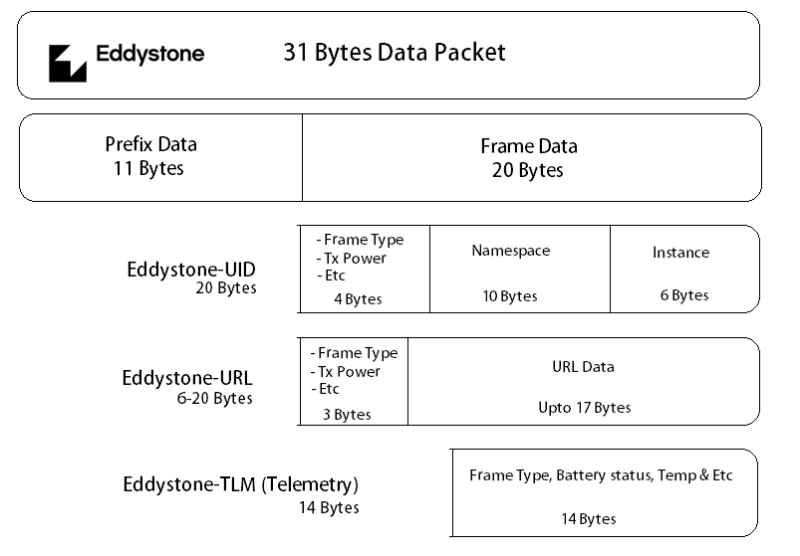
\includegraphics[width=.6\textwidth]{figures/eddystoneProtocol.png}
\caption[abs]{Tipos de paquetes Eddystone con su respectivo tamaño.\\
{\scriptsize (Fuente: \citep{protocolosBeacon})}}
\label{fig:eddystone}
\end{figure}

\begin{figure}[ht!]
\centering
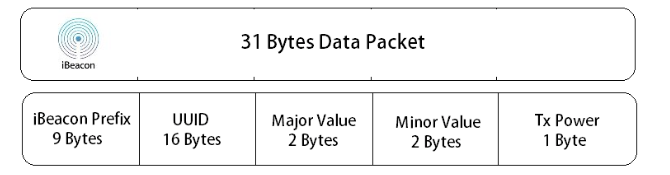
\includegraphics[width=.6\textwidth]{figures/ibeaconProtocol.png}
\caption[abs]{Paquete IBeacon realizado por Apple.\\
{\scriptsize (Fuente: \citep{protocolosBeacon})}}
\label{fig:ibeacon}
\end{figure}

\section{Estabilidad de la señal Bluetooth}

Las señales u ondas de radio son altamente afectadas por ruido o interferencia presente en el entorno, perdiendo asi intesidad en la señal o resultando en valores fluctuantes que causan estimaciones o eventos no esperados. Esto ocurre por ejemplo en las interferencias de señales Wi-Fi al descargar un archivo, o también en equipos Bluetooth al conectarse a un equipo de musica. La localizacion en interiores al depender igualmente del valor de Received Signal Strength Indicator( RSSI) o intensidad de la señal recibida; se ve ampliamente afectado, sobre todo por el hecho de que los usuarios estan caminando y en un entorno cambiante. El RSSI habitualmente se expresa en en dBm para medir la potencia obtenida por una señal recibida. Su valor mayor teorico es 0 dBm y la escala corresponde a valores negativos, en donde mas negativo implica una mayor perdida de señal.

El cuerpo humano asi como otros objetos, provoca una perdida de señal debido a la atenuacion de esta, debido a la reflexión o refracción que ocurre segun los materiales en donde la señal incide. El cuerpo humano provoca absorcion de las señales y disminución de la calidad de estas. Ademas, la propagación multicaminos es un efecto latente en todas las ondas de radio, en donde las ondas llegan al receptor por diferentes caminos y diferentes tiempos, provocando interferencia constructiva o destructiva. Este fenómeno habitualmente ocurre por los medios en donde se transportan las ondas y el entorno como tal, provocando que la señal obtenida difiera de la original manifestando ruido e interferencia, disminuyendo asi la calidad e intensidad de esta.

Para corroborar como afectan estos fenómenos a la intensidad de la señal recibida por Beacons Bluetooth, se realiza una prueba en donde se pueden visualizar los efectos de obstruccion en la señal. Para realizar esta prueba se utiliza un telefono celular con una pequeña aplicacion la cual es capaz de percibir las señales Bluetooth emitidas por un dispositivo Beacon en sus cercanías. Cada cierto tiempo se registran los valores RSSI percibidos y se escriben en un archivo de texto para posteriormente ser procesados. Se mide la señal durante 3 minutos con una linea de visión limpia, es decir, sin obstrucciones o interferencias entre ambos dispositivos. Luego, una persona camina entre la linea de visión y también permanece quieto en ella, obstruyendola completamente. La \autoref{fig:beacon_interferencia} muestran los resultados de estas pruebas.

\begin{figure}[ht!]
\centering
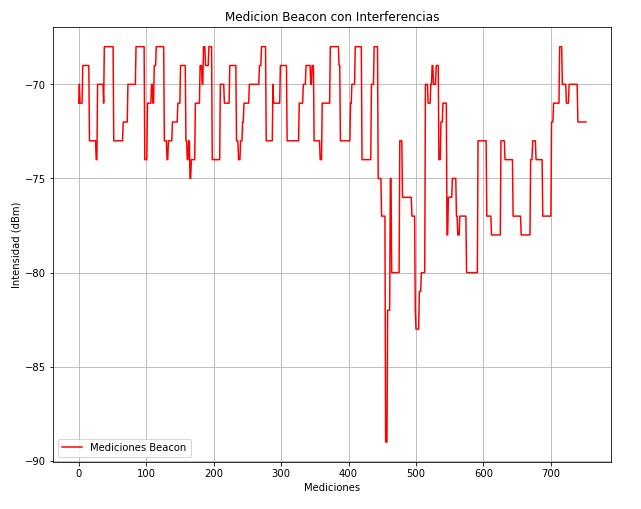
\includegraphics[width=.6\textwidth]{figures/mediciones_beacon_interferencia.jpg}
\caption[abs]{Resultados del cambio en la señal producto de una persona caminando delante de la linea entre un Beacon y un teléfono celular receptor\\
{\scriptsize (Fuente: Elaboración propia)}}
\label{fig:beacon_interferencia}
\end{figure}

Como se observa en la imagen, en un principio, la señal oscila en valores inferiores a -75 dBm, lo cual es aceptable y medianamente bueno según la escala RSSI. Posteriormente a partir de la medición 400, se introduce la aparición de la persona en la linea de propagación de la señal, con lo que inmediatamente la intensidad de la señal se reduce significativamente, incluso llegando a los limites de -90 dBm que es básicamente inestable, ya que para una conexión segura al menos se recomienda -80 dBm. Posteriormente la persona se mueve a través de la linea de visión, provocando los efectos de la gráfica, es decir, señales intermitentes y poco estables.

Todo esto demuestra principalmente que no se puede confiar completamente en el valor de la intensidad de la señal recibida, ya que es muy probable que arribe con efectos de multicamino u obstrucciones que modifican su valor durante el viaje. Este efecto es significativamente mayor en grandes distancias de viaje en las señales, lo cual sugiere que los Beacons instalados no tengan una disposicion tan distante, es decir, para obtener mejores resultados es mucho mejor una gran densidad de Beacons por superficie, lo que aumenta el costo de despliegue. Por otra parte los algoritmos de posicionamiento deben aprender a leer e interpretar este ruido, basado en patrones segun la posicion, con lo cual los algoritmos supervisados de maquinas de aprendizaje son sumamente efectivos en este ámbito.

\section{Evaluación y selección de Beacons Bluetooth}
\label{sec:seleccion}

A pesar de que en el mercado existe una gran variedad de empresas proveedoras de beacons bluetooth, hay dos que se destacan por sobre los demás y que son pioneras dentro de esta industria, estas son Estimote \citep{estimote} y Kontakt \citep{kontaktio}. Amas empresas proveen de hardware y soluciones de software ya implementadas y listas para el uso empresarias o pequeños desarrollos. Para compararlos solo se considerar los beacons estandar dentro de cada proveedor, ya que existen multiples variedades en cada segmento, sin embargo estos poseen otras cualidades como sensores de luz, temperatura, lectores NFC, UWB, o son resistentes al agua, polvo, entre otros. Para hacer un análisis justo y conciso, en este caso se obviaran estas características aunque si pueden ser utilizadas en diversos contextos. 

Para la comparativa se utilizan las características indicadas por cada fabricante y estas se resumen en la siguiente tabla:

\begin{table}[]
\centering
\caption{My caption}
\label{my-label}
\begin{tabular}{|c|c|c|}
Parametro                   & Kontakt.io                      & Estimote                             \\ \hline
Duracion de la bateria      & Hasta 4 años                    & Hasta 2 años                         \\ \hline
Rango                       & 70m                             & 70m                                  \\ \hline
Procesador                  & 32-bit ARM® Cortex™ M0 CPU core & ARM® Cortex®-M4 32-bit processor FPU \\ \hline
Sensibilidad                & -93dBm                          & -96 dBm                              \\ \hline
Velocidades                 & 250kBs, 1Mbs, y 2Mbs            & 1 Mbps (2 Mbps soportado)            \\ \hline
Memoria                     & 256KB flash 16KB RAM            & 512 kB Flash memory 64 kB RAM memory \\ \hline
Transmission power          & -30dBm to 4dBm                  & -20 to +4 dBm                        \\ \hline
Bateria                     & 2 x 1.000mAh CR2477             & 1 x CR2477 – 3.0V                    \\ \hline
Bluetooth                   & Bluetooth® 4.2 LE standard      & Bluetooth® 4.2 LE standard           \\ \hline
Espesor                     & 15mm                            & 17mm                                 \\ \hline
Peso                        & 35 gr                           & 30 gr                                \\ \hline
Paquete ibeacon y eddystone & 1 a la vez                      & 1 a la vez                           \\ \hline
Paquetes adicionales        & telemetria                      & telemetria                           \\ \hline
Sensores adicionales        & Temperatura                     & movimiento, temperatura              \\ \hline
Bateria reemplazable        & Si                              & Si                                   \\ \hline
Numero de beacons           & 3                               & 3                                    \\ \hline
Precio                      & 60 USD                          & 59 USD                               \\ \hline
\end{tabular}
\end{table}

La tabla (numero de tabla) muestra que ambos equipos son muy similares en teoría, ademas ambos presentan kits de desarrollo de software para las principales plataformas, ya sea web, aplicaciones móviles como Android e IOS como también permiten la integración de la infraestructura en la nube. Para determinar entonces la elección, es necesario realizar pruebas en ambos hardware, sin embargo estas pruebas ya han sido realizadas en múltiples ocasiones por investigadores como se aprecia en \citep{comparativaKontakt} en donde se realizaron pruebas de fluctuación en las señales para ambos equipos. La prueba consiste en poner beacons kontakt y estimote a una distancia de 2 metros de un dispositivo móvil que registra la señal. Ambas configuraciones son idénticas en los equipos y las mediciones fueron realizadas cada 500ms. Los resultados de las pruebas indican que los beacons de Kontakt tienen muchas menos fluctuaciones y la señal permanece estable por mucho mas tiempo, lo que es un indicio que pueden ser mucho mas factibles en la localización en tiempo real.


\section{Algoritmos de \textit{Machine Learning}}

Para determinar la posición del dispositivo móvil, es necesario contar con un algoritmo que pueda inferir la posición del usuario basado en las señales percibidas por los distintos Beacon. Para ello en este trabajo se utilizaran los denominados algoritmos de aprendizaje automático o \textit{machine learning}. En términos generales los algoritmos de aprendizaje automático corresponde a una rama de la inteligencia artificial en donde su objetivo principal es lograr que los computadores puedan aprender por si mismas, sin necesidad de programar su comportamiento explicitamente. Para lograr esto, se entrenan los diferentes algoritmos mediante información suministrada en forma de ejemplos según el tipo de resultado que se espera. El auge de este tipo de técnicas ocurre con la llegada del internet y los grandes volúmenes de datos, ya que para resolver ciertos problemas como clasificación de imágenes, los algoritmos convencionales son NP-Hard, es decir, su complejidad computacional es muy alta o desconocida, por lo tanto no es computacionalmente computable en un tiempo razonable, por lo que las técnicas de aprendizaje automático o heuristicas pueden entregar resultados positivos con una alta precisión sin necesidad de programar un algoritmo especifico a cada problema.

Para la utilización de estos tipos de técnicas, es necesario una representación adecuada de los datos acorde al problema que se requiere resolver, para ello se deben describir los datos, por ejemplo los pixeles de una imagen como una matriz de atributos, es decir, cada registro o fila es una imagen y cada atributo, campo o columna de la matriz es un pixel de la imagen. La representacion de los datos es de vital importancia para obtener unos resultados positivos.

Dentro del aprendizaje automático se distinguen dos tipos de técnicas de las mas conocidas, las cuales son aprendizaje supervisado y no supervisado. El aprendizaje supervisado corresponde a deducir una función o mapeo según los datos con los cuales es entrenado el modelo, para ello al momento de entrenar se debe suministrar pares de objetos, en donde una componente son los datos de entrada, por ejemplo los pixeles de una imagen; y en la segunda componente se suministra la clase de esta imagen, que puede corresponder por ejemplo al objeto presente en la imagen, como un tipo de animal o automóvil, dependiendo del problema a tratar. Entonces la función es capaz de determinar un valor numérico (regresión) o una etiqueta(clasificación) para nuevos datos no vistos anteriormente. Por lo anterior, es necesario que el modelo generalice adecuadamente y no se sobre ajuste a los datos de entrenamiento, es decir, solo sea capaz de inferir correctamente sobre el conjunto de entrenamiento y no para nuevos datos. Mientras mas datos son suministrados, mas fácilmente es para las técnicas de aprendizaje automático predecir correctamente para nuevos datos.

Estos algoritmos son tipicamente implementados en dos fases. En la primer fase, denominada fase de entrenamiento o \textbf{training phase}, los datos son recopilados y manipulados de forma tal que pueden ser suministrados a los algoritmos de aprendizaje automatico, de esta forma, los algoritmos pueden ``aprender" patrones de los datos y clarificarlos. En la segunda fase, denominada fase de pruebas o \textbf{testing phase}, nuevos datos no vistos previamente son probados en el algoritmo entrenado en la primera fase, para dilucidar la efectividad del modelo construido.

A lo largo de este trabajo se utilizan muchos tipos de algoritmos, sin embargo a continuación se procede a describir los mas relevantes y que serán mayormente utilizados en la localización en interiores, ya que a lo largo de investigaciones previas han demostrado buenos resultados en problemas similares.

\begin{figure}[ht!]
\centering
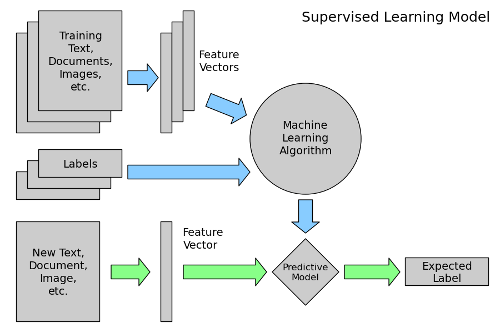
\includegraphics[width=.6\textwidth]{figures/image_machinelearning.png}
\caption[abs]{Esquema básico del funcionamiento de las técnicas de aprendizaje automático\\
{\scriptsize (Fuente: \cite{machineLearningBasic})}}
\label{fig:machineLearningBasic}
\end{figure}

\subsection{K-Nearest Neighbor}

El método K-Nearest Neighbor o método de los \textbf{k} vecinos mas cercanos, abreviado también como \textbf{\textit{k-nn}} es un metodo d eclasificacion y regresion supervisada, muy simple pero a la vez poderoso, ya que es no parametrico, es decir, no es necesario configurar parámetros del modelo, por lo que entradas de datos similares deben tener salidas de datos similares. Este método estima la funcion de densidad $F(\frac{x}{C_{j}}$ de las predictorias $x$ (datos de entrada) por cada clase $C_{j}$. En el proceso de aprendizaje no se hace ninguna suposición sobre el la distribución de las variables predictorias.

Aunque es un algoritmo supervisado, su fase de entrenamiento es muy acotada, enfocandose mayormente en la fase de pruebas, ya que todo el esfuerzo realizado por este algoritmo es hecho sobre la marcha, es decir, mientras se ejecuta estima la mejor prediccion en cada instante de la fase de entrenamiento, por lo que también se habla de un algoritmo de aprendizaje basado en instancias.

Los datos son representados por vectores en un espacio multidimensional, en donde cada ejemplo posee $p$ atributos y existen $q$ clases para clasificarlos. Luego el algoritmo esencialmente separa el espacio multidimensional en regiones, en donde un nuevo dato sera clasificado como perteneciente a una clase $C$ siempre y cuando esta clase sea la mas frecuente entre los $k$ vecinos mas cercanos al dato en cuestión. Para medir la distancia entre datos o vectores, se puede utilizar distancia euclideana, manhattan, Chevyshev, distancia del coseno, entre otras. Luego, por ejemplo para la distancia euclideana se tiene la siguiente formula:

\[ d(x_{i}, x_{j}) = \sqrt{\sum_{r=1}^{p}(x_{ri} -x_{rj})^{2}} \]

Luego, un dato esta descrito como:

$$ x_{i} = (x_{1i}, x_{2i}, ..., x_{pi}) \in X$$

Luego la fase de entrenamiento del algoritmo consiste en almacenar los valores y sus características, así como las etiquetas. En la fase de clasificacion, se mide la distancia entre el nuevo vector y los datos de entrenamiento previamente almacenados y se seleccionan los $k$ ejemplos mas cercanos, para posteriomente ser clasificado segun la clase que mas se repite dentro del conjunto de elementos seleccionados.

Este algoritmo tiene un problema al suponer que todos los atributos son igualmente relevantes, ya que al usar la distancia euclideana, todos valen lo mismo, por lo que un atributo relevante tiene el mismo ``peso'' que uno irrelevante. Sin embargo este problema no ocurre en la clasificación utilizando Beacons, ya que cada una de las señales emitidas por distintos Beacons es igual de relevante y no importa su peso.

Un problema relevante al tratar con algoritmos basados en distancia es el llamado efecto de la ``maldicion de la dimensionalidad'' o \textit{curse of dimensionality}, el cual hace referencia al problema de encontrar patrones en espacios de altas dimensiones, ya que mientras mas alta es la dimensionalidad de los datos, mas dispersos están y para seguir obteniendo resultados buenos, es necesario suministrar una cantidad de datos que crece exponencialmente. Ademas, al ser tan grande el espacio dimensional, es mucho mas complejo encontrar patrones o regiones para lograr una correcta clasificación.

Por ultimo, al tener muchos atributos, y muchos datos de entrenamiento, k-nn se torna muy lento, ya que para inferir un nuevo dato de prueba, requiere recorrer todos los datos de entrenamiento, provocando que el tiempo de procesamiento aumente significativamente a medida que aumenta el numero de datos en el \textit{dataset}. Esto es un punto relevante en el posicionamiento indoor, ya que en un simple despliegue de una infraestructura de Beacons por ejemplo en un centro comercial, se deben almacenar miles de puntos de referencia, con lo cual k-nn puede reducir su \textit{performance} y demorar demasiado, lo cual es critico en posicionamiento en tiempo real.

La \autoref{fig:knn} muestra el funcionamiento de k-nn y como el valor seleccionado de $k$ puede afectar en la clasificación.

\begin{figure}[ht!]
\centering
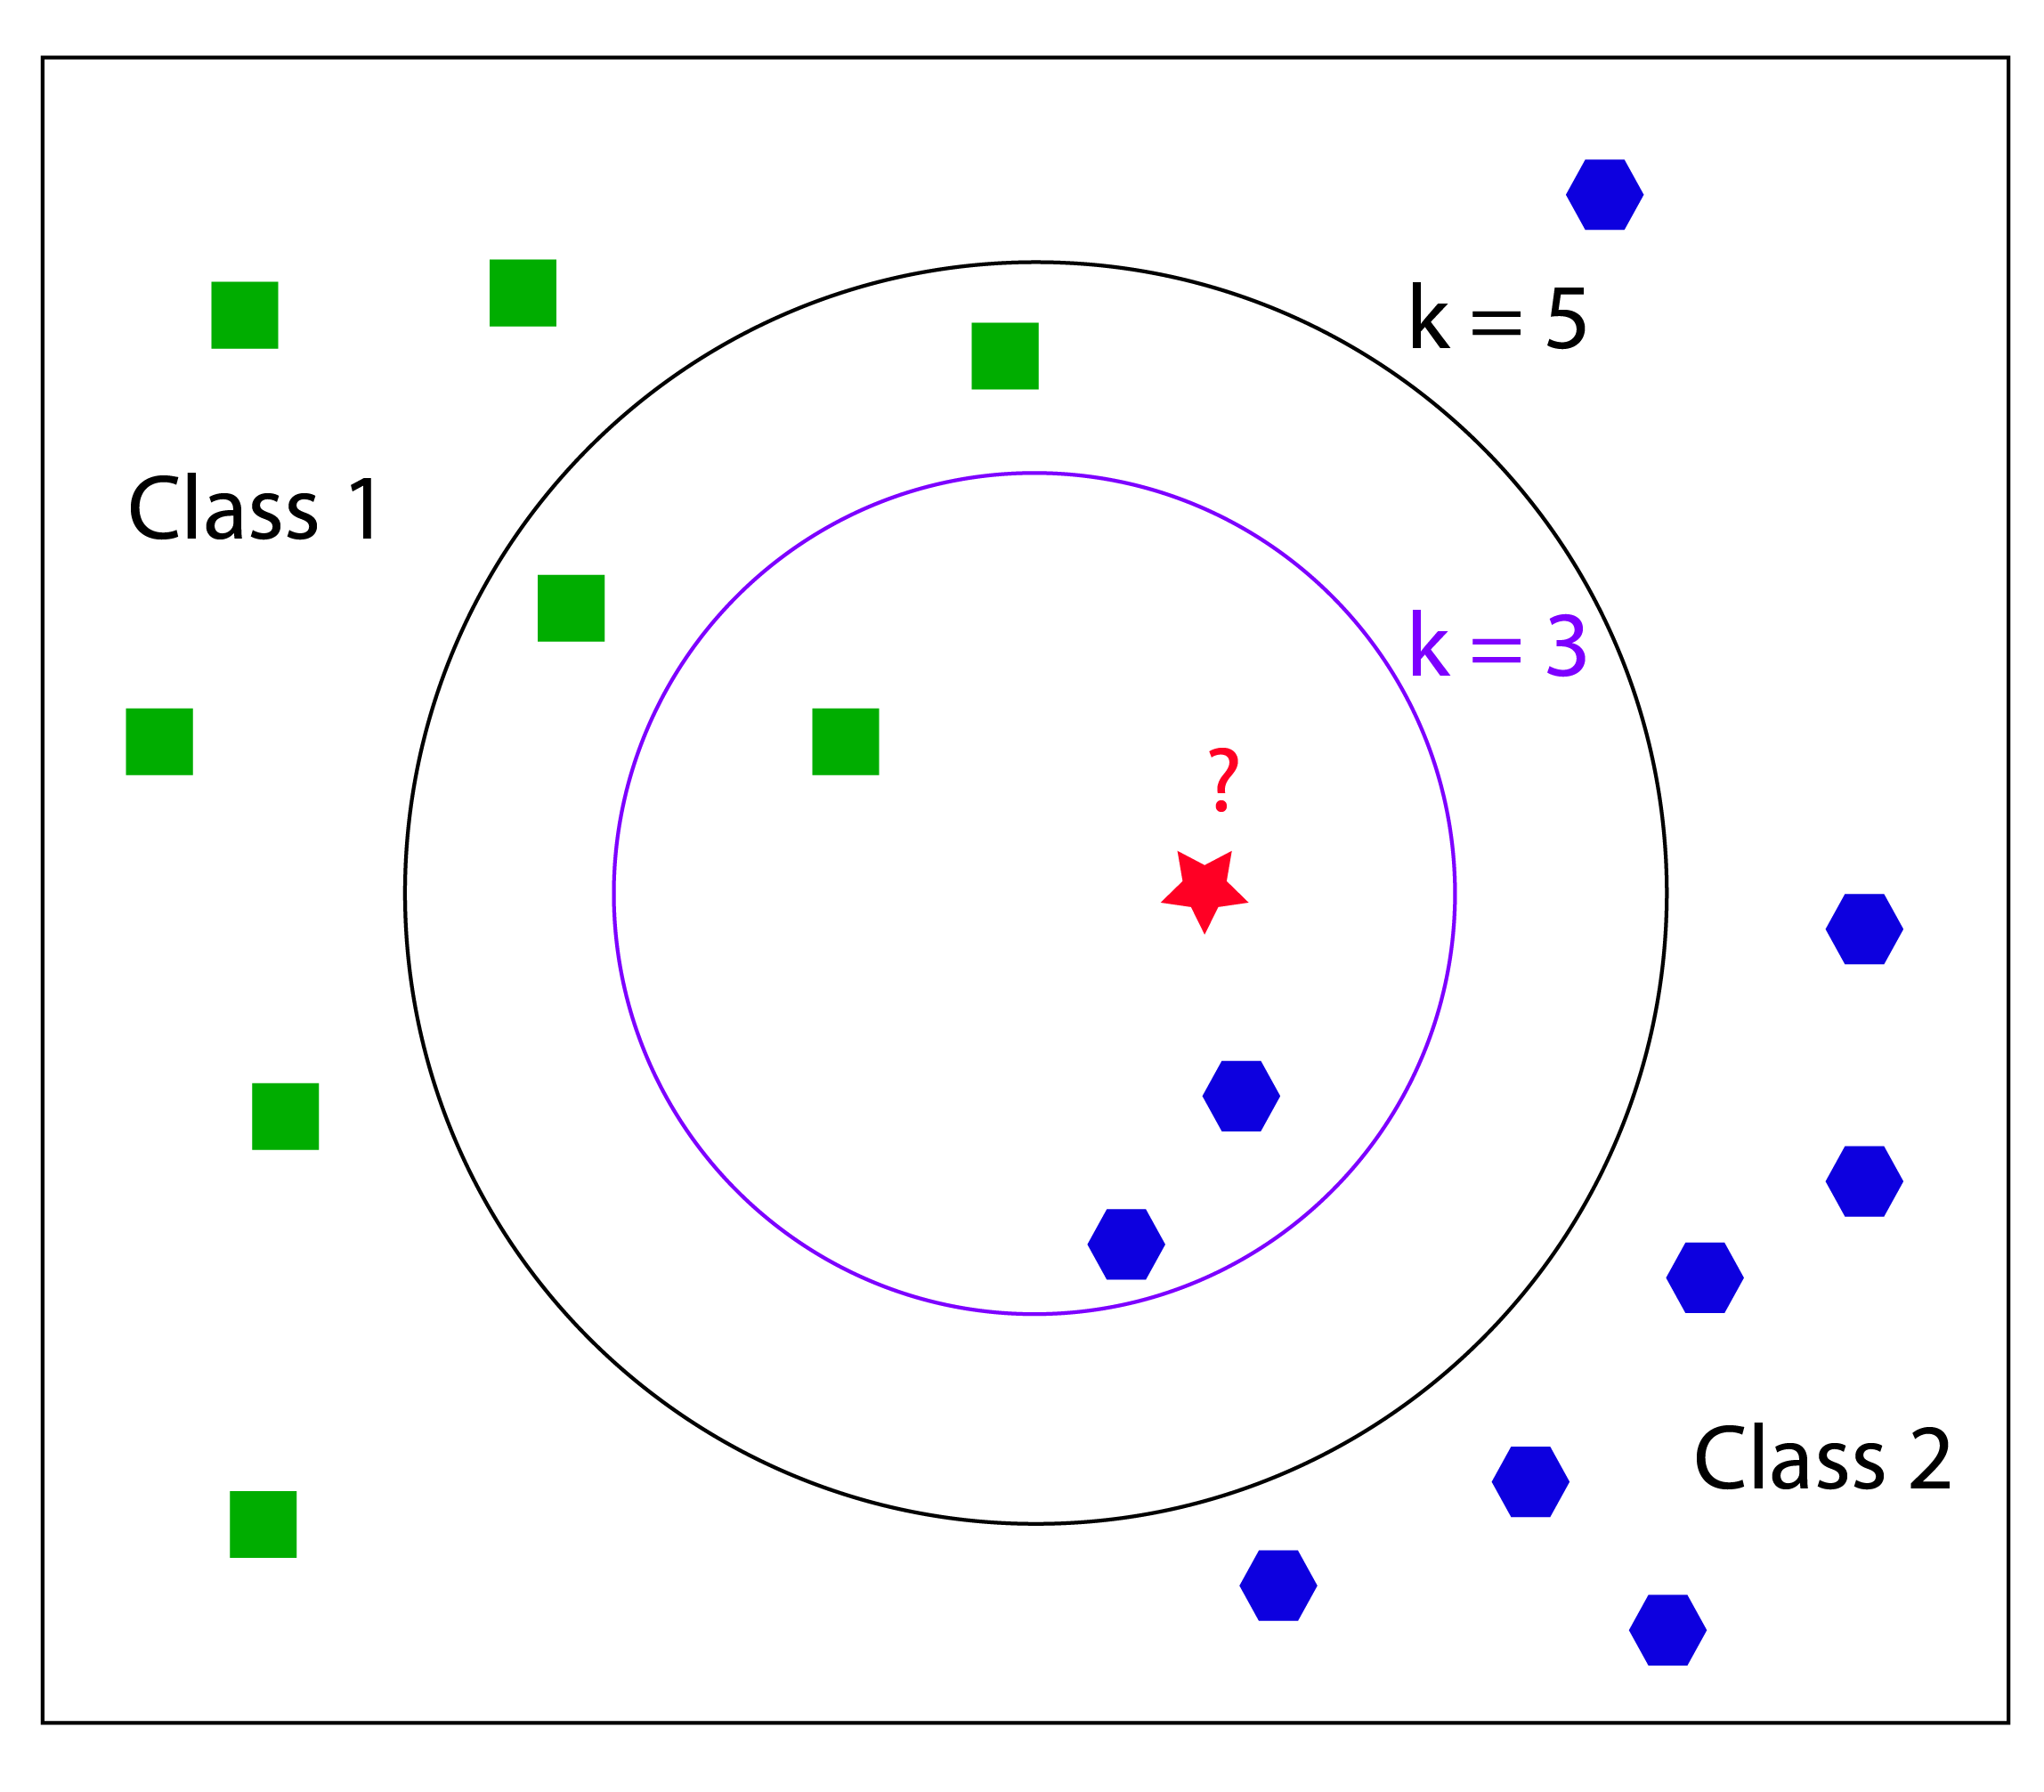
\includegraphics[width=.6\textwidth]{figures/knn.png}
\caption[abs]{Ejemplo de clasificación utilizando k-nn con $k=5$ y $k=3$}
\label{fig:knn}
\end{figure}

\section{Support Vector Machines}

Otro de los algoritmos mas utilizados en aprendizaje supervisado corresponde al denominado \textit{support vector machine}(SVM) o maquina de vectores de soporte. Ese algoritmo es sumamente utilizado sobre todo en problemas de clasificación, regresión y \textit{detección de outliers}. Una maquina de vectores de soporte construye un hiperplano o un conjunto de ellos, en un espacio de alta dimensionalidad o dimensionalidad infinita, el cual puede ser utilizado para clasificación. Intuitivamente, un buen hiperplano separador es aquel que logra maximizar la distancia a cada ejemplo de entrenamiento mas cercano a el, de cada clase, lo cual se conoce como margen funcional, entonces mientras mas grande es este margen, menor es el error de generalización del clasificador, es decir, permite mayor generalización para nuevos datos sin definir un margen estricto que solo se adapte a los datos de entrenamiento. Posteriormente para clasificar nuevos ejemplos, la SVM ubica este nuevo punto en una región del espacio que corresponde a una clase, segun su distancia y posicion respecto al hiperplano definido en la fase de entrenamiento.

\begin{figure}[ht!]
\centering
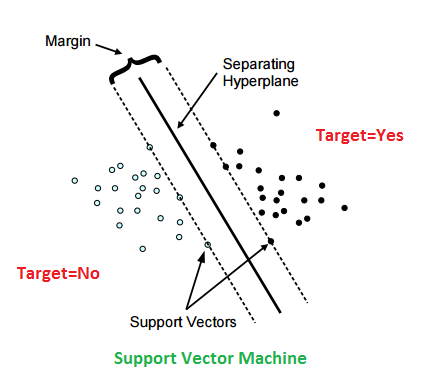
\includegraphics[width=.6\textwidth]{figures/SVM-Planes.png}
\caption[abs]{Ejemplo SVM en dos dimensiones, en donde se muestran los vectores de soporte y el hiperplano que logra la máxima separación}
\label{fig:svm}
\end{figure}

Como muestra la \autoref{fig:svm}, este hiperplano logra una separación en un espacio de dos dimensiones, lo cual es adecuado en clasificación binaria. Aunque la formulación matemática es idéntica, para resolver SVM en problemas de multiclases, es necesario escoger un esquema de resolucion. Una de las aproximaciones mas utilizadas de resolucion es reducir el problema de multiclasificacion en muchos problemas de clasificacion binaria. Para ello se utilizan formulaciones conocidas en la inteligencia artificial como \textit{one-vs-all} o es quemas de votos como \textit{one-vs-one}. La formulación matemática se muestra a continuación:

Dado un conjunto de vectores de entrenamiento $x_{i} \in I\!R ^{p}, \rm i = 1, ..., n$ en dos clases y un vector $ y  \in \{1, -1\}^{n}$ , SVM resuelve el siguiente problema de optimizacion:

$$ \underset{w, b, \zeta}{\mathrm{min}} \, \frac{1}{2} w^{T}w + C
\sum_{i=1}^{n} \zeta_{i}$$

sujeto a: 

\begin{align}
y_{i} ( w^{T} \phi(x_{i}) + b \geq  1 - \zeta_{i}, \\ 
\zeta_{i} \geq 0, \\
i = 1, ... , n
\end{align} 

En su forma dual de problema de programacion lineal, este problema es puede ser expresado como:

$$ \underset{\alpha}{\mathrm{min}} \, \frac{1}{2} \alpha^{T} Q \alpha - e^{T} \alpha$$

sujeto a: 

\begin{align}
y^{T} \alpha = 0, \\
\quad 0\leq \alpha_{i} \leq C, \, i = 1, ..., n 
\end{align} 

En donde $e$ es el vector de unos, $ C > 0$ es el limite superior, y $ Q$ es una matriz semidefinida positiva de tamaño $ n$ por $ n$, $ Q_{ij} = y_{i} y_{j} K(x_{i}, x_{j})$ en donde $K(x_{i}, x_{j}) = \phi(x_{i})^{T} \phi(x_{j})$ se denomina el kernel y es sumamente importante en SVM, ya que este permite llevar desde un espacio en donde la separación de las clases no es tan clara, a un espacio de dimensiones muy grandes o infinitas, en donde la separación se vuelve mucho mas obvia.

Finalmente, la función de decisión corresponde a:

$$ sgn(\sum_{i=1}^{n}y_{i} \alpha_{i}K(x_{i}, x) + \rho)$$ 

La relevancia del kernel es lo que torna a SVM muy factible en problemas de clasificación, ya que permite llevar los datos de un espacio finito, en donde no son linealmente separables, a un espacio de dimension infinita en donde si pueden ser separados linealmente, lo cual es conocido como \textit{kernel-trick}. Ademas, como solo se utilizan funciones kernel que utilicen producto punto, la operación de llevar estos datos al nuevo espacio es eficiente y de bajo costo computacional. Para realizar el kernel trick, cada producto punto es reemplazado por una funcion kernel de carácter no lineal. El kernel mas utilizado es RBF o radial basis function el cual es definido como:

$$ K(x_{i}, x_{j}) = exp(- \gamma \left\|{ x_{i} - x_{j}}\right\|^2) , \, \gamma > 0$$

Luego, utilizando este kernel, se debe escoger el parametro $\gamma$ y el parametro $ C$ adecuado, los cuales son muy importantes en una correcta generalización del SVM. Habitualmente SVM al ser un hiperplano de máxima distancia a cada clase, es muy estricto en la clasificación, lo cual no siempre es lo ideal, debido a que pueden existir \textit{outliers} debido a ruido, afectando a toda la clasificación. El hiperparametro $C$ ayuda en este sentido, con lo que se denomina \textit{soft-margin}, es decir, un margen mas permisivo, que clasifica de manera errónea algunos ejemplos de entrenamiento, buscando la generalización del SVM.

Por otra parte, el hiperparametro $\gamma$ define que tan lejos alcanza la influencia de un ejemplo de entrenamiento por si solo, es decir, puede ser visto como el inverso del radio de influencia de los ejemplos de entrenamiento escogidos como vectores de soporte. Un valor pequeño de $\gamma$ producirá un largo alcance, definiendo zonas de clasificación muy amplias, con lo cual no se aprecia completamente la forma o patrón de estas. Por otra parte un valor grande, provoca demasiada separación, aislando cada ejemplo de entrenamiento.

\section{Redes Neuronales y Deep learning}

Uno de los campos de investigación con mayor auge en el ultimo periodo, es todo lo relativo a los avances en redes neuronales, particularmente \textit{deep learning}.  La base de estos modelos computacionales son, como indica su nombre, las neuronas y su funcionamiento en el cerebro y el sistema nervioso. El cerebro, en particular el sistema visual o corteza visual primaria, es el responsable de reconocer patrones, y lo hace de manera tal en que una imagen es dividida y analizada a traves de muchas capas, disminuyendo la complejidad en cada una de ellas para ir de lo macro a lo micro, pudiendo asi establecer patrones de menor escala y localidades en la imagen que ayuda a distinguir de que se trata el objeto visualizado.

Cada unidad neuronal esta conectada a las neuronas de la capa siguiente y ellas pueden aumentar o inhibir el estado de las neuronas en la capa siguiente. Estos sistemas por lo mismo, pueden aprender solos, solo se debe suministrar un numero adecuado de ejemplos para el entrenamiento.

Cada activacion de la neurona en la capa siguiente depende de los pesos $w$ y el sesgo o \textit{bias} $b$. Los pesos multiplican a las entradas en cada conexion, y el bias es el limite, de donde se establece si la suma ponderada de las entradas con los pesos es mayor o menor que el bias, entonces la neurona se activa.

\begin{figure}[ht!]
\centering
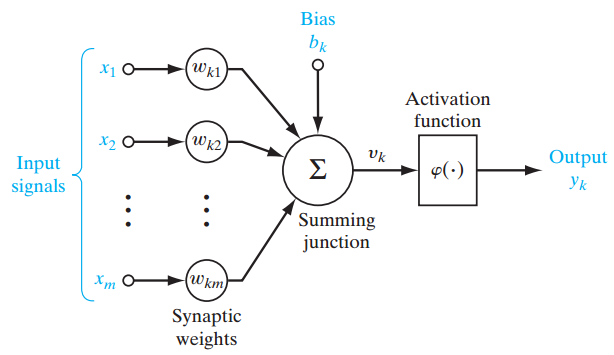
\includegraphics[width=.6\textwidth]{figures/SLP.png}
\caption[abs]{Esquema basico de single layer perceptron\\
{\scriptsize (Fuente: \cite{slp})}}
\label{fig:slp}
\end{figure}

La \autoref{fig:slp} muestra como cada entrada es multiplicada por su respectivo peso, y la suma ponderada se suma con el bias, para luego utilizar la funcion de activacion y obtener la salida , la cual describe que tanto aporta esta neurona, la cual sera el nuevo input para la siguiente capa. La neurona perceptron queda descrita como:

\begin{equation}
output = \left\{ \begin{array}{lcc}
             0 &   si  & w \cdot x + b \leq 0 \\
             \\ 1 &  si & w \cdot x + b > 0 \\
             \end{array} \right.
\end{equation}

En donde $ w\cdot x = \sum_{j} w_{j} x_{j} $ con $w$ y $x$ son vectores en donde sus componentes son los pesos y las entradas respectivamente, y el numero de neuronas en la capa corresponde a $j$. A pesar que este modelo sirve para problemas simples, no funciona de buena manera en problemas altamente no lineales. 

La neurona mas utilizada es la denominada neurona sigmoid. Estas neuronas son similares a las neuronas perceptron(primeras neuronas inventadas), pero pequeños cambios en sus pesos y sesgos, provocan pequeños cambios en las salidas, lo cual las hace mucho mas útiles y diversifican muy bien la información a través de la red. La funcion de activacion de este tipo de neuronas corresponde a la funcion sigmoid, y ayuda a resolver problemas estrictamente no lineales. Luego el output $y_{k}$ viene dado por:


$$ \sigma( w \cdot x + b) = \frac{1}{1 + exp(- \sum_{j} w_{j}x_{j} - b)}$$

Luego el procedimiento por el cual aprende la red corresponde a un algoritmo denominado \textit{backpropagation} el cual puede computar los pesos y bias adecuados para la red, con el objetivo de entrenarla y definir los mejores hiperparametros para posteriomente clasificar de manera correcta nuevos ejemplos. El algoitmo de backpropagation consiste en los siguientes pasos:

\begin{enumerate}
\item \textbf{Input:} Iniciar la correspondiente activación de la capa de entrada

\item \textbf{Feedforward:} Computar las salidas de cada neurona de las capas ocultas. Finalmente computar la salida de la capa de salida.

\item \textbf{Output error:} Computar los errores de la capa final o capa de salida

\item \textbf{Backpropagation:} Propagar el error de la capa de salida a la capa anterior oculta. Repetir para todas las capas hasta llegar a la capa de entrada.

\item \textbf{Output:} Calcular el gradiente de la función de costo, para luego actualizar los pesos y bias.

\end{enumerate}

Para calcular el gradiente se utiliza gradiente descendente, y entonces, cada iteracion consiste en atravesar la red hacia adelante, computar el error y volver para propagar el error y computar los ajustes y actualizaciones a los hiperparametros. Este algoritmo ha logrado un gran avance en las redes neuronales artificiales permitiendo entrenarlas de manera mucho mas rápida, logrando grandes resultados.

Las redes neuronales obtienen buenos resultados en gran parte de los problemas, pero para problemas demasiado complejos el concepto de multilayer perceptron, es decir, el modelo estandar de redes neuronales, no es suficiente. Para ello, ha surgido el concepto de \textit{deep learning} o aprendizaje profundo. Estas redes son similares a las redes normales, pero poseen mas de una capa escondida y ademas se han desarrollado otros algoritmos para resolverlas eficientemente. 

\begin{figure}[ht!]
\centering
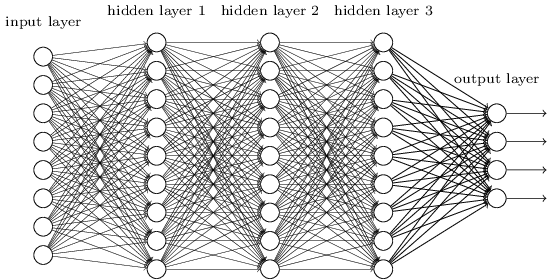
\includegraphics[width=.6\textwidth]{figures/deep.png}
\caption[abs]{Red neuronal profunda con multiples capaz escondidas\\
{\scriptsize (Fuente: \cite{slp})}}
\label{fig:slp}
\end{figure}

Para resolver este tipo de redes profundas existen muchos acercamientos, y cada día nacen nuevas formas de resolución. Las formulaciones matemáticas son muy extensas, pero en términos generales los algoritmos de backpropagation y gradiente descendente son las bases fundamentales de resolución, a pesar que necesitan modificaciones para que la red no se quede atascada en ciertas capas, cosa que habitualmente ocurre en redes profundas.

\section{Descripción del \textit{framework} de posicionamiento}

Para la elaboración del sistema de posicionamiento, se utiliza la técnica de fingerprint discutida en el estado del arte, la cual mediante la utilización de un mapa de señales, también denominado \textit{radiomap}, puede inferir la posición de un usuario utilizando algún algoritmo de localización. Como el objetivo de este trabajo es determinar los mejores algoritmos de maquinas de aprendizaje para posicionamiento indoor utilizando bluetooth low energy, es necesario establecer un marco de trabajo mediante el cual se pueda llevar a cabo esta tarea.

Lo primero a tener en consideración, es que se deben utilizar dispositivos Bluetooth Low Energy, lo cuales realizan la función de access point(AP) y que serán los responsables de emitir la señal RSSI. Luego, el procedimiento se divide en las dos clásicas etapas de fingerprint, es decir, fase \textit{offline} y fase \textit{online}

\subsection{Fase Offline}

Para la generación del radiomap, se debe crear un tipo de aplicación que sea capaz de recolectar los vectores RSSI en diversos puntos dentro del lugar de experimentación. Esta aplicación debe ser simple y permitir la adición de nuevos puntos fingerprint. Por lo tanto, esta es una tarea muy importante, ya que estos datos se implementaran los algoritmos de maquinas de aprendizaje. El periodo y frecuencia de los datos se debe determinar experimentalmente. Para ello, cada punto a colectar, representa un punto en el espacio $2-dimensional$, es decir, un punto dentro del plano. Para generar la grilla, es necesario tener la posicion exacta, que corresponde a la etiqueta de cada punto mapeado. Entonces, se formara una grilla de múltiples puntos con sus respectivos fingerprints leídos. Cabe destacar que los puntos de referencia en donde se toman los datos, no necesariamente deben estar equiespaciados, pero de esta manera es mucho mas simple formar la grilla, ya que cada punto de medición puede corresponder al centro de un cuadrado de determinadas dimensiones. La \autoref{fig:fingerprints} muestra la grilla a desarrollar, con un punto de referencia y su respectivo vector RSSI expresado en dBm.

\begin{figure}[ht!]
\centering
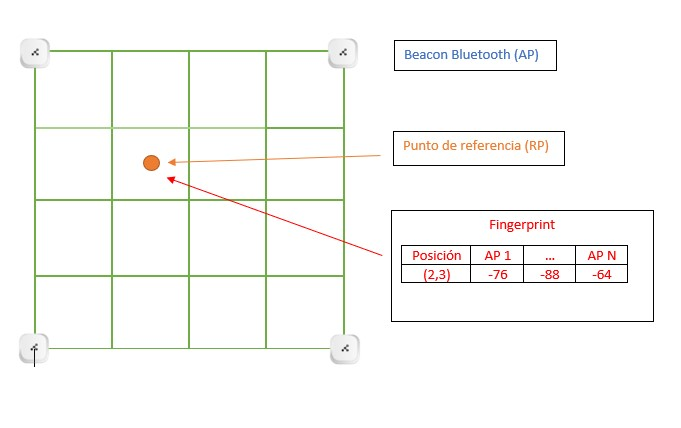
\includegraphics[width=.6\textwidth]{figures/fingerprints.jpg}
\caption[abs]{Ejemplo de grilla utilizada, con sus puntos de referencia y los fingerprints leidos, que corresponden a vectores de señales RSSI\\
{\scriptsize (Fuente: Elaboración propia)}}
\label{fig:fingerprints}
\end{figure}

Con los datos registrados, se debe crear la base de datos que almacenara estos fingerprints, ya que desde ahí es posible analizar los datos y mantener su persistencia. Posteriormente, con estos datos se crea el radiomap respectivo, es decir, asociar un vector de señales RSSI, en donde cada componente representa la intensidad recibida proveniente de un access point, a cada posicion en donde se colectaron los datos. El numero de fingerprints depende del numero de posiciones en donde se colectan los datos, y también de cuantos ejemplos se obtienen en cada una de estas posiciones. La tabla ejemplifica la estructura del radiomap a contruir:

\begin{table}[]
\centering
\caption{My caption}
\label{my-label}
\begin{tabular}{|c|c|c|c|c|}
\hline
Posicion & AP 1 & AP 2 & ... & AP N \\ \hline
(3,3)    & -65  & -70  & ... & -95  \\ \hline
(6,6)    & -80  & -50  & ... & -76  \\ \hline
\end{tabular}
\end{table}

Cabe destacar que los algoritmos de maquinas de aprendizaje a pesar que pueden resolver para problemas multivariados, es decir, predecir para dos variables, en este caso $(x,y)$ como un punto; es mucho mas sencillo separar esto en dos problemas, vale decir, un algoritmo de maquina de aprendizaje para $x$ y otro para $y$. Otra alternativa seria asociar una clase a cada punto, es decir, numerar estos puntos de la grilla, pero el problema con esto es que se torna mucho mas complejo de aprender, debido a que se necesitarían demasiados datos para verdaderamente lograr un aprendizaje de cada una de estas clases, provocando un aumento significativo en la complejidad del problema.

Teniendo en consideración los puntos anteriormente mencionados, el siguiente paso es entrenar los algoritmos de aprendizaje a ser comparados y utilizados en el posicionamiento. Antes de el entrenamiento, es necesario de destacar que se utilizara un algoritmo de reducción de dimensional. Esto no ha sido mayormente explorado en la literatura, sin embargo puede ser de mucha utilidad a la hora del entrenamiento y la fase \textit{online}. La principal razón de utilizar estas técnicas, es que los puntos de referencia poseen una alta correlación, debido a que la onda decae según el cuadrado de la distancia, por lo que se presenta una correlación entre dos puntos adyacentes. Por otra parte, los métodos de extracción de características, pueden ayudar a agilizar la fase de entrenamiento, ya que este proceso es lento. Ademas, al ser menos componentes, en la fase online, las técnicas tardaran mucho menos tiempo en determinar la posición en tiempo real, lo cual es sumamente efectivo en técnicas como KNN.

Existen dos métodos muy conocidos mediante los cuales se puede reducir la dimensionalidad, estos son \textit{Linear discriminant analysis}(\textbf{LDA}) y \textit{principal component analysis}(\textbf{PCA}). Por un lado LDA es una tecnica habitualmente utilizado en los campos de estadisticas, reconocimiento de patrones y maquinas de aprendizaje. El objetivo de LDA es encontrar una combinación lineal de los \textit{features} o caracteristicas del dataset, las cuales separan dos o mas clases. La combinacion lineal resultante es habitualmente utilizada como clasificador o mas popularmente para reducir la dimensionalidad del dataset. LDA es similar a PCA, ya que ambos buscan combinaciones lineales que explican de mejor manera los datos, sin embargo la manera en que los realizan es diferente, ya que LDA explicitamente intenta modelar la diferencia entre las clases de datos, por lo que necesita de las etiquetas de cada clase, lo cual lo torna un metodo supervisado. Por otro lado, PCA no toma en cuenta la diferencia entre las clases, por lo que es un metodo no supervisado. Ademas LDA funciona bien en el caso de que las variables o atributos del dataset son independientes, y predicen la variable categorica o etiqueta de cada clase.

Como se menciono anteriormente, LDA maximiza la separación entre clases, es decir, la varianza entre clases o interclases. PCA por su parte, busca las componentes de la combinación lineal, las cuales maximizan la varianza en los datos, esto quiere decir, la varianza de las variables o varianza intraclases. LDA hace presunciones sobre los datos que lo vuelven mas complejo de implementar, por ejemplo, las clases deben estar normalmente distribuidas, y la covarianza de las clases debe ser igual. Por todo lo anterior, y como es necesario reducir la correlación entre los puntos adyacentes, se decide utilizar PCA como tecnica para reducir el espacio de dimensionalidad y para encontrar un espacio no correlacionado de variables. Esto es necesario, debido a que al estar tan correlacionado los puntos de referencia en la grilla, puede existir información o \textit{features} escondidos, lo cual no aumentara la \textit{accuracy} de las técnicas de machine learning, pero si mejora los tiempos de entrenamiento y en la fase online, lo cual es muy relevante en un sistema de posicionamiento en tiempo real. La correlación se debe a que como es sabido, las ondas se propagan de la siguiente forma:

$$ I \propto \frac{1}{r^{2}}$$

En donde $I$ representa la intensidad y $r$ es la distancia de propagación desde el punto de emision. Esta formula define como decae la intensidad de la señal a medida que esta se transmite en el medio según el inverso del cuadrado de la distancia. Con lo anterior, y considerando que los Beacons actuan como antenas omnidireccionales, si el RSSI de dos Beacons se mide en un punto, luego se translada a otro punto adyacente, y se mide nuevamente,  al ser la intensidad proporcional a la distancia, ambos Beacons y sus lecturas mantienen una correlación lineal, ya sea positiva o negativa, ya que ambos aumentan o disminuyen en un mismo valor según la distancia obtenida, siempre y cuando esta sea pequeña o ambas señales se propaguen en la misma dirección espacial en un vecindario determinado. Esto se conoce tradicionalmente como correlación espacial de las señales.

Como la técnica elegida es PCA, a continuación se procede a describir como funcionara específicamente para el problema de fingerprint. PCA, busca la proyección sobre la cual los datos queden mejor representados en términos de mínimos cuadrados. Esta convierte un conjunto de variables posiblemente correlacionadas en un conjunto de variables sin correlación lineal, las cuales se denominan componentes principales. PCA construye una transformacion lineal que escoge un nuevo sistema de coordenadas para el conjunto original de los datos, escogiendo la varianza mayor de los datos como primera componente en el nuevo sistema de referencia, la segunda varianza mas grande como segunda componente y asi suscesivamente. Para ello se requiere la matriz de covarianzas, mediante la cual es posible encontrar los vectores propios de la misma, que funcionan como base para las nuevas coordenadas a traves de la transformacion lineal y asi reducir la dimensionalidad.

PCA resuelve el problema de la alta dimensionalidad del radiomap construido, combinando los \textit{features} mediante una transformacion lineal en un espacio no correlacionado, es decir, un espacio ortogonal de vectores( vectores propios), utilizando la matriz de covarianza de los datos de entrenamiento de tamaño $ N \, x \, N$ . Luego, este radiomap de señales RSSI es proyectado en el espacio no correlacionado en la dirección de la varianza mas alta. La seleccion respectiva de componentes principales se basa en las varianzas mas grandes, es decir, segun los valores propios mas grandes (proyeccion de la transformación). Por lo anterior, los valores propios representan la información de las componentes principales.

El espacio característico es generado mediante un conjunto de $M$ lecturas RSSI por posición o punto de referencia, lo cual corresponde a un vector $x_{i}$ de tamaño $ M \, x \, 1$ como vector columna, donde $ M$ es menor a $ N$, y con $ N$ el numero de ejemplos de entrenamiento.

Luego, el espacio característico posee una media:

$$ \overline{x} = \sum_{i=1}^{N} \frac{x_{i}}{N} $$

Por ende, la matriz de covarianzas puede ser descrita como:

$$ C_{r} = \sum_{i=1}^{N} (x_{i} - \overline{x})(x_{i} - \overline{x})^T = X_{i}X_{i}^T$$

Cabe destacar que la matriz de covarianzas es simetrica y de tamaño $N \, x \, N$, por lo cual posee $N$ valores propios.

Sean los valores propios $ \{ \lambda_{1}, \lambda_{2}, ..., \lambda_{N} \} $ ordenados en orden descendiente, con sus correspondientes vectores propios normalizados $ \{ V_{1}, ... , V_{N} \} $ . Según la formula de valores y vectores propios para matrices debe cumplirse entonces:

$$ C_{r} V_{i} =  \lambda_{i} V_{i}$$
$$ \lambda_{1} \geq \lambda_{2} \geq ... \geq \lambda_{N}$$

Como se menciona anteriormente, los vectores propios $ \{ V_{1}, ... , V_{N} \} $ son no correlacionados y ortonormales, por lo que forman un espacio característico.

Con todo lo anterior, es posible proyectar el radiomap en el nuevo espacio característico. Obviamente, si se proyecta sobre todas las componentes no existe un cambio, ya que se presenta la misma información, por lo cual es necesario determinar los valores propios mas relevantes y que aportan mayor información(varianza) a los que no. Para la selección entonces de las componentes principales se toma en cuenta entonces la información contextual y el error que cada componente ha aportado. No existe manera automática de determinar el numero adecuado de componentes principales, sin embargo en la experimentación es discutida una forma de poder llevar a cabo esta tarea. 

Luego, el nuevo radiomap no correlacionado $Z_{i}$ es calculado proyectando $X_{i}$ en el espacio característico reducido $W$, el cual representa una combinación lineal de los vectores propios seleccionados, asociados a los valores propios mas relevantes. Finalmente, la matriz $Z$ del nuevo radiomap, con menor numero de componentes esta dada por:

$$ W = X \, x \, V$$

$$ Z_{i} = W^{T} \, x \, X_{i} \quad \forall i$$

Luego, los clasificadores de maquinas de aprendizaje son entrenados mediante la utilización del radiomap $Z$, el cual tiene componentes reducidas y no dependientes, con lo cual el entrenamiento es mucho mas rápido y se elimina la mayor parte de la información redundante al extraer la información mas relevante.

Las principales ventajas de utilizar PCA entonces, corresponde a \citep{7743586}:

\begin{enumerate}
\item PCA extrae la información importante del radiomap definido.

\item PCA reduce la matriz de datos multivariados sin perder mucha información, en donde los datos están descritos por muchas variables correlacionadas dependientes.

\item PCA reduce la complejidad mediante la disminución del numero de componentes, logrando mejorar tiempos de entrenamiento y calculo online.
\end{enumerate}


El siguiente paso entonces corresponde a entrenar los modelos definidos, que se explican en la parte experimental, los cuales son técnicas de maquinas de aprendizaje muy conocidos y que han presentado buenos resultados a lo largo de muchos problemas. Posteriormente, se seleccionan los mejores algoritmos, es decir, que presenten el mejor desempeño y son implementados. Una parte importante a definir en la etapa offline, es la manera en que los modelos de machine learning funcionaran en el dispositivo, ya que hay dos versiones posibles de implementacion, estas son utilizando un servidor o sin utilizar servidor. 

Ambas estrategias deben entrenar los algoritmos en una maquina dedicada, por el consumo de recursos que son necesarios, sin embargo una vez que los modelos estan entrenados, deben ser utilizados en el dispositivo movil. Para ello se puede exponer un servicio REST o API en donde el dispositivo movil envia una nueva lectura RSSI al servidor, posterior a esto el servidor computa y determina la posición y retorna este valor al dispositivo móvil. Esta alternativa es ideal en entornos donde siempre existe conexion a internet y redes de telefonía e internet movil. Esta alternativa es idonea, ya que es el servidor quien procesa los resultados, haciendo el posicionamiento mas expedito, ademas de utilizar menos recursos en el telefono y por lo mismo menos batería, ya que solo realiza conexiones de red de poco peso(solo transmite un vector de enteros).

En el caso de este trabajo, como se pretende utilizar en lugares donde no existe internet como mineras o estacionamientos subterráneos, la alternativa es desarrollar el entrenamiento en el servidor, pero luego portar los modelos a un dispositivo móvil. Esto es posible, debido a que la mayoria de los modelos desarrollados presentan ciertos componentes que pueden ser posteriormente replicados en otras maquinas sin necesidad de entrenar o re entrenar el modelo. 

Todos los pasos anteriores describen a grandes rasgos el proceso completo de la etapa offline, desde la recolección de datos hasta el entrenamiento e implementacion de los modelos en los dispositivos móviles.

\subsection{Fase Online}

Para la fase online se reconocen dos etapas principales, la primera es colectar un vector de señales RSSI en la posición actual del usuario, es decir, el vector de intensidad de la señal en donde cada componente representa la intensidad recibida por un Beacon o Access Point Bluetooth. La segunda etapa es proveer este vector de entrada a los algoritmos de aprendizaje supervisado. Para realizar esta tarea se deben tener en cuenta las normalizaciones realizadas y aplicar correctamente la transformación PCA del espacio característico antes de suministrar los datos a los algoritmos, ya que de otra manera las dimensiones serán incompatibles.

Para realizar esto, se debe proyectar el vector RSSI en el espacio característico de la ecuación xx, es decir $W$. Los valores proyectados en esta etapa son comparados con los modelos entrenados buscando de esta manera el valor estimado mas cercano según el nuevo radiomap. Una vez que los algoritmos de clasificación proveen el resultado de la posición física, entonces la misma aplicación de la fase offline, es utilizada para mostrar en un mapa de tiempo real la localización actual de usuario.

La fase Online es muy simple, ya que solo se deben evaluar los nuevos valores en los algoritmos, por lo que es claro que la parte mas importante de todo el proceso de fingerprint es la recoleccion adecuada de datos y el correcto entrenamiento de los algoritmos de \textit{machine learning}. Esto es de suma importancia, ya que malos datos o malos parámetros de entrenamiento, eventualmente provocan problemas hacia adelante, es decir, reducir la precisión en la fase Online afectando severamente los resultados.

A continuación, la \autoref{fig:propuesta} describe el procedimiento completo a desarrollar en este trabajo.


\begin{figure}[ht!]
\centering
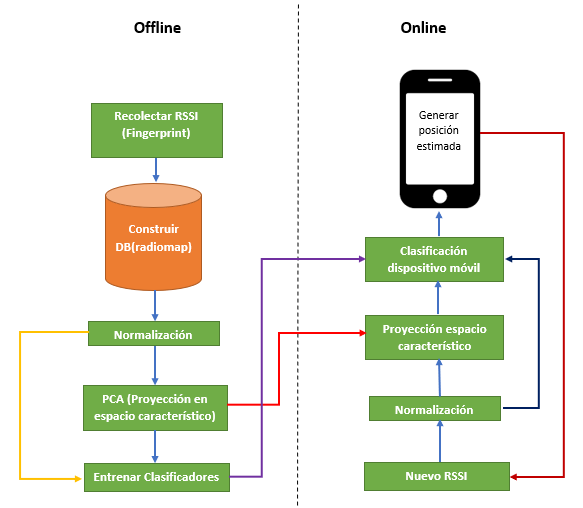
\includegraphics[width=.6\textwidth]{figures/propuesta_memoria.png}
\caption[abs]{Framework desarrollado para resolver el problema de posicionamiento en interiores\\
{\scriptsize (Fuente: Elaboración propia)}}
\label{fig:propuesta}
\end{figure}

Como se observa en la \autoref{fig:propuesta}, los datos son normalizados previamente antes de ser utilizados. Ademas la razon de la conexion entre la normalizacion y el entrenamiento de los clasificadores se debe a que se utilizaran los algoritmos de machine learning utilizando PCA y no utilizándolo, a modo de comparación en términos de tiempo y accuracy. Ademas, se ha omitido el item en donde los clasificadores ya entrenados son portados al dispositivo movil. Finalmente, hay que notar que en la fase online, el dispositivo movil genera un nuevo vector de señales RSSI, luego se transforman los datos y finalmente se clasifican, lo que genera una posicion estimada que se refleja en el dispositivo móvil. Este ciclo es constante, ya que la posición se actualiza continuamente según los parámetros definidos y frecuencia de actualización.